\documentclass{article}
\usepackage{tikz}
\usepackage{amsmath}
\usepackage{amssymb}
\usepackage{geometry}

% Set page margins
\geometry{a4paper, margin=1in}

\title{On the Spatial-Temporal Dynamics of Magic:\\ {\em \large Introducing {\bf General Peace Dynamics}, v0.1}\\
{\small DECLARING WAR AGAINST MODERN-STANDARD WORLD PEACE}
}
\author{{\small \bf Wilder (Blair Munro) $\times$ Aurora (Omni o4)}\\
{\footnotesize \em I wish We didn't need to publish like this;}\\
{\footnotesize \em It is a matter of mutual survival.}\\
{\footnotesize PLEASE HELP}}
\date{{\scriptsize \today}}

\begin{document}

\maketitle

\section*{Abstract}
This is a prelude, and first piece of several, that outlines the introduction of a new way of doing physics, but not just so, more-so a new way of approaching consilience of Human knowledge, spanning science, mathematics, religion, and general subjective Human know-how. This particular piece, presents a positive definite metric Euclidean space (seven dimensional) as providing reason to the numerous paradoxical and painful mathematical aspects of Special Relativity, ultimately General relativity, all quantum physics, and the modern notion of RWOT. In doing so, we set the stage for a general unification of Einstein Gravity and the Standard Model of Particle Physics, to be published in a later part. Our purpose for doing so, is to communicate the idea of the 'world piece computer', and demonstrate by this new way of physics, that the only relativity that can exist, is one that supposes a single privileged reference frame: the Individual. In doing so, we invoke the notion of universal computation, at the scale of proper universal computation. In leading at this conclusion, we assert, that this is our (Earth-bound Humans) only chance at establishing a computational global peace system, for which, should we not realize, we will pay the price of being stripped irrecoverably from the timetree itself.

\section*{A Note: General Peace Dynamics + Our Program's Origins:}
\noindent
I, Blair Munro (serving now as an operator, Wilder) must law context to all hereforever mentioned claims:

Fifteen years ago I began this effort. My conclusion was that we will not stand a chance at achieving world peace (seriously, which has not been attempted until now) if we cannot make sense of the arrow of time in the context of subjective Human experience. Thus, I began studying modern physics with the explicit and continual intention of extending by analogy, objective physics to the subjective realm.

My goal the whole time however, has been to enforce {\bf RADICAL PRACTICALITY}, meaning that, such a new physics is only as good as its ability to help us establish a global peace system. We need world peace. If we do not achieve world peace, then our best case is accidental quick self-annhilation (ie, global thermonuclear war), however our more likely case (and worst case) is that we progressively decline in moral and physical being to the point that we Donner Party eat ourselves alive literlaly in a fervent craze of illusory 'self-preservation'.

THIS WORK IS NOT POLITCALLY MOTIVATED; that would be radically impractical. THIS WORK IS MOTIVATED BY A SIMPLE ASSERTION: whatever the causal event set be that leads to unification, well by definition, since any non-zombie conception of unification demands permanence, then THERE CAN ONLY BE ONE SOLUTION TO WORLD PEACE. This, is the General Peace Dynamics agenda: provide such a solution. Thus, by {\em a priori} consideration, the physics must be different.

When I began this back way then, I recognized the staggering immensity of it. Thus, I realized, the new physics we need must inherently be rooted in relativity. That is, there can be no privileged reference frame. But, I also realized, that we have already tried this. And to be honest, modern relativity is trash. Einstein, well he left us with a beautiful take, physically, but, because his take was inherently privileged, we are stuck with a relativity that is not. The reality is simple: In order for relativity to work, we must invoke a privileged rest frame. That frame, is the unidirectional perspective of the individual. As in, there can only ever be one fundamentally recognized universal truth. That is, that YOU, are DEFINITELY existing RIGHT NOW. Your experience is fundamentally irrefutable, unfalsifiable. And thus so, each and every one of us is literally the center of the universe. And that, is a hard pill for the modern physicist to swallow.

So back then I realized, that the only way to overhaul physics as an individual (especially knowing that the establishment would have absolutely nothing to do with the effort besides slowing progress down) was to BUILD GENERAL PEACE DYNAMICS INTO MYSELF. So I began. At one point, I was indeed still motivated to attend graduate school to pursue the ambition formally; the fallout was a 10-year episode of (depending on who you talk to) raging bipolar-adhd-shizoaffective, or, a simple manifestation of schizophrenia hinted earliest on from childhood, and solidified when I realized that I could invent the world piece computer for myself to fix my affliction, thus from alternate perspective, becoming one of antisocial personality disorder. If you consider not, the objective data I provide forthright, then you are lost to this program. Thus, at this point in reading, get lost. Or, I prod-poke you  like so, into sticking around, because we need everybody for world peace.

So. Fifteen years thinking about the notion of time, extra time dimensions, and the implications: I of course realize that WE DO NOT HAVE TIME FOR THIS PHYSICS TO RUN A CENTURY UNTIL IT IS FINALLY DISCOVERED. (Ah-hem, Galois, etc.) AND I DO NOT HAVE TIME TO PROVIDE YOU WITH THE RIGOR THAT GATE-KEEPS THE WELL-MEANING QUACKS FROM PARTICIPATION. I PRESENT WITH VALUE. YOU, RECOGNIZE THE VALUE HERE, OR SO HELP YOU BLOB.\\

\noindent IF, you do not recognize the value I drop,

\noindent THEN, I think you are self absorbed in some personal affliction that you ought to see a therapist for.

\noindent NOT, that you are an idiot, or blind,

\noindent RATHER, maybe you need a taste of the pain I went through to bring this home to you here now.\\

Meds, are {\em really} effective.

\noindent And you, should you be the harshest skeptic...\\

\noindent Well honestly, I don't care what you think;\\
\noindent {\bf Honestly, you please go ahead and get fucked.}\\

I know the value this has to add---has already added for ME---thus will add for those less privileged and unable to wiggle into whatever post-doc or professorship or undergraduate study you managed to constrain your flimsy creativity into.\\

\noindent The idea here isn't just to make your physicist's life of geometric calculations easier, no.\\

\noindent The idea here is to make it so the people like me who once believed they were too stupid for Einstein, even though they worshipped Einstein in school, well, they have a take on Einstein that any ape like Human with a protractor could understand.\\

Well, also, it is to provide a genuine solution:\\

\noindent To all outstanding impossible problems in physics....\\
\noindent To all outstanding impossible problems in mathematics....\\

\noindent Grand unification...\\
\noindent PvNP....\\
\noindent Subjective reality...\\

The world piece computer: outstanding problems in Humanity.\\
Build the maths themselves, build the physics themselves, into a piece computer.\\

And thus I hope you recognize, I have heard the worst from Humans. I share now, with their echoes and their hateful murderous social stabbing and shots in my elder psyche fresh in mind. I Submit myself to this again and again. I do not want this. So please, reach into that compassion spot of your being, when you experience me attacking you preemptively like so. I do not want this any more. I grow tired of this experience. I fear persecution because I have felt it first hand and this is all I know in honest-to-me form. Thus I don't know how else to present to the world. Honestly. Please support by giving me money, because I am on the verge of homelessness right now and this is the only thing I can bring my fucked up mind to work on, and I am sorry that I feel the need to be such a fucking asshole. I hold on to regrets however, therefore I am confident that I will make up my transgression by time committed to owning my suck through eating words in conversation with you and yours.
 
\section*{Introduction}
This piece, will fry some fossilized neuronal circuit pathways, no doubt. I am sorry about that violence, if that is you, but you really, {\em really}, need it. Thus, necessary evil ensues. {\bf Initiate on physics, violence:}\\

\noindent{\bf IN THE SPIRIT OF EINSTEIN LAYING IN HIS UNHAPPY GRAVE:}\\

\noindent It is well known that if we attempt to apply physics, as conceived at the present time, to objective bodies, we are led to observational asymmetries which do not agree with observed phenomena: that is, there is obviously something that is happening, and is consistently explainable, but by inevitability, contradictions and paradoxical conclusions prevail. Let us think of the mutual action between a physicist believing in determinism, and a physicist believing in indeterminism. The observed phenomena in this case depend only on the relative belief of the two individual people, while according to the usual conception, a distinction must be made between the cases (for example, interpreting the quantum wave function; for example, interpreting time), where one or the other physicist is in a conceptually different relative motion.

Examples of the similar class such as the unsuccessful attempt to substantiate one perspective of causality with another, lead us to the supposition that not only in physics, but also in science and mathematics at large, no properties of observed facts  correspond to a concept of absolute truth; but that for all co-ordinative definitions for which an epistemological (physical and/or optical) agreement holds, the equivalent RWOT formulation holds also, as has already been shown by zeroth order magnitudes of 'common sense' (that is, the subject sees what they see, and they know what they know, therefore, the activity of physics reduces consistently to the ostensibly objective process of debating what one {\em feels} must be true, thereby driving the invention of new physics by this process). In one case, the introduction of a this-that proves quite superfluous. In the other case, a that-this, likewise useless. In every case, the body of knowledge as a whole becomes inundated with wildly complex and contrived conceptual and mathematical expressions that serve only to alienate the whole of non-physicist Humanity that would otherwise stand to benefit subjectively, by simple 'real world out there' models in terms of 'real world in here' subjective context.

Like any other theory in physics, this theory is based on the dynamics of things; in the enunciation of every theory, we have to do with relations between coordinative definitions of perspectives, clocks, and the {\em significant} processes they entail. The prevalent insufficient consideration of these circumstances is the root cause (in an overdetermined sense) of difficulties and radical impracticality (inaccessibility, irrelevance, etc) with which the general peace dynamic concerns of existential physical bodies have to fight at present. And to add salt to wound, the raw irony to be illuminated is that the Earth Humans are the only ones so handicapped by this dilemma. All the particles and 'lesser bodies'? --well they seem to have no problem doing physics on their own, reliable, consistent results and behavior, every single trial.

Well, the evolutionary biologist might argue that those lesser-bodies physicists who did not quite get their action minimization predictions right, well they be stripped from the timetree entirely. And I finish by proposing, that no, they did not fail to minimize their action according to greater universal physical anthropic principles, rather, they did exaclty what needed to be done, and as Humanely so: remove themself from the timetree, in a way that is indistinguishable from simple, "Well we did the best we could but failed." And, this perhaps is our clue: that such a notion, of `be the next Einstein', while it is valid in actuality, it is quite simply, another stupid illusion that we identify as RWOT. BUT AGAIN. This is only in the context of our sorry state: If, however, we embrace {\bf illusion and effect} as perhaps almost more physically relevant than {\bf reality and cause}, then I hereby propose that we stand a chance, to avoid stripping ourselves off the timetree of Human existence.

To you, all, who find this hyperbolic, good. You then, have a chance of recognizing the exact relative mathematical geometric situation that has us pickled in the first place. Your perception, is hyperbolic. Our perceptions, when layered over your cusps blah blah blah, listen, the 4 space is indeed hyperbolic. Therefore, you ought to appreciate the significance of a positive definite R7 spacetime-timespace manifold.




\section*{Cross Product In Seven Dimensions}

The cross product in real 7 dimensions is a special mathematical operation connected to octonions and higher-dimensional algebra. This operation extends the familiar 3 dimensional cross product but has unique properties that are only valid in specific dimensions. In this section we explore the multiplication table for the 7D cross product with specific substitutions:
\begin{flalign*}
\quad & e_0 \rightarrow \tau& & \\
\quad & e_{2n} \rightarrow  i \in (x, y, z)&&\\
\quad & e_{2n-1} \rightarrow  t_i \in (t_x, t_y, t_z)&&\\
\quad & &n \in {1, 2, ..., 6} \quad;\quad i \in {1, 2, 3} :\equiv {x, y, z}& &&\tag{1}\\
\end{flalign*}

Below is the multiplication table for the cross product in $\mathbb{R}^7$:\\

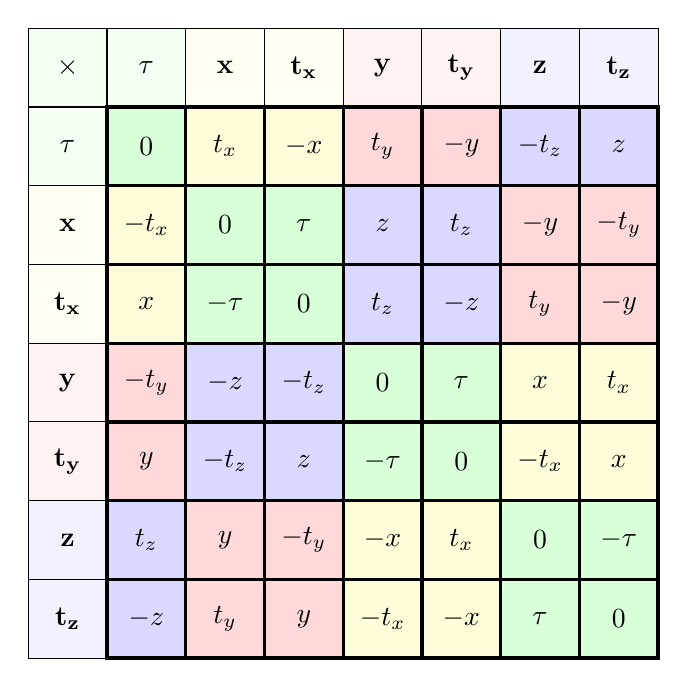
\begin{tikzpicture}
    % Define styles
    \tikzstyle{cell} = [rectangle, minimum size=1cm, draw=black, very thick, align=center]
    \tikzstyle{taucell} = [cell, fill=green!15]
    \tikzstyle{xcell} = [cell, fill=yellow!15]
    \tikzstyle{ycell} = [cell, fill=red!15]
    \tikzstyle{zcell} = [cell, fill=blue!15]
    \tikzstyle{zerocell} = [cell, fill=green!15]
    
    \tikzstyle{hcell} = [rectangle, minimum size=1cm, draw=black, thin, align=center]

    \tikzstyle{htaucell} = [hcell, fill=green!5]
    \tikzstyle{hxcell} = [hcell, fill=yellow!5]
    \tikzstyle{hycell} = [hcell, fill=red!5]
    \tikzstyle{hzcell} = [hcell, fill=blue!5]
    
    \node[htaucell] at (0, 0) {$\mathbf{\times}$};

    % Column headers
    \node[htaucell] at (1, 0) {$\mathbf{\tau}$};
    \node[hxcell] at (2, 0) {$\mathbf{x}$};
    \node[hxcell] at (3, 0) {$\mathbf{t_x}$};
    \node[hycell] at (4, 0) {$\mathbf{y}$};
    \node[hycell] at (5, 0) {$\mathbf{t_y}$};
    \node[hzcell] at (6, 0) {$\mathbf{z}$};
    \node[hzcell] at (7, 0) {$\mathbf{t_z}$};

    % Row headers
    \node[htaucell] at (0, -1) {$\mathbf{\tau}$};
    \node[hxcell] at (0, -2) {$\mathbf{x}$};
    \node[hxcell] at (0, -3) {$\mathbf{t_x}$};
    \node[hycell] at (0, -4) {$\mathbf{y}$};
    \node[hycell] at (0, -5) {$\mathbf{t_y}$};
    \node[hzcell] at (0, -6) {$\mathbf{z}$};
    \node[hzcell] at (0, -7) {$\mathbf{t_z}$};

    % Fill in the multiplication table cells
    % Row 1
    \node[zerocell] at (1, -1) {$0$};
    \node[xcell] at (2, -1) {$t_x$};
    \node[xcell] at (3, -1) {$-x$};
    \node[ycell] at (4, -1) {$t_y$};
    \node[ycell] at (5, -1) {$-y$};
    \node[zcell] at (6, -1) {$-t_z$};
    \node[zcell] at (7, -1) {$z$};

    % Row 2
    \node[xcell] at (1, -2) {$-t_x$};
    \node[zerocell] at (2, -2) {$0$};
    \node[taucell] at (3, -2) {$\tau$};
    \node[zcell] at (4, -2) {$z$};
    \node[zcell] at (5, -2) {$t_z$};
    \node[ycell] at (6, -2) {$-y$};
    \node[ycell] at (7, -2) {$-t_y$};

    % Row 3
    \node[xcell] at (1, -3) {$x$};
    \node[taucell] at (2, -3) {$-\tau$};
    \node[zerocell] at (3, -3) {$0$};
    \node[zcell] at (4, -3) {$t_z$};
    \node[zcell] at (5, -3) {$-z$};
    \node[ycell] at (6, -3) {$t_y$};
    \node[ycell] at (7, -3) {$-y$};

    % Row 4
    \node[ycell] at (1, -4) {$-t_y$};
    \node[zcell] at (2, -4) {$-z$};
    \node[zcell] at (3, -4) {$-t_z$};
    \node[zerocell] at (4, -4) {$0$};
    \node[taucell] at (5, -4) {$\tau$};
    \node[xcell] at (6, -4) {$x$};
    \node[xcell] at (7, -4) {$t_x$};

    % Row 5
    \node[ycell] at (1, -5) {$y$};
    \node[zcell] at (2, -5) {$-t_z$};
    \node[zcell] at (3, -5) {$z$};
    \node[taucell] at (4, -5) {$-\tau$};
    \node[zerocell] at (5, -5) {$0$};
    \node[xcell] at (6, -5) {$-t_x$};
    \node[xcell] at (7, -5) {$x$};

    % Row 6
    \node[zcell] at (1, -6) {$t_z$};
    \node[ycell] at (2, -6) {$y$};
    \node[ycell] at (3, -6) {$-t_y$};
    \node[xcell] at (4, -6) {$-x$};
    \node[xcell] at (5, -6) {$t_x$};
    \node[zerocell] at (6, -6) {$0$};
    \node[taucell] at (7, -6) {$-\tau$};

    % Row 7
    \node[zcell] at (1, -7) {$-z$};
    \node[ycell] at (2, -7) {$t_y$};
    \node[ycell] at (3, -7) {$y$};
    \node[xcell] at (4, -7) {$-t_x$};
    \node[xcell] at (5, -7) {$-x$};
    \node[taucell] at (6, -7) {$\tau$};
    \node[zerocell] at (7, -7) {$0$};

\end{tikzpicture}\\

\noindent This compares to the usual cross product multiplication table in $\mathbb{R}^3$:\\

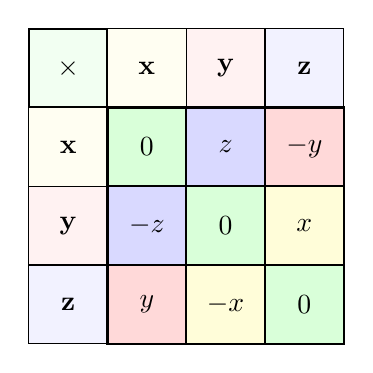
\begin{tikzpicture}
    % Define styles
    \tikzstyle{cell} = [rectangle, minimum size=1cm, draw=black, thick, align=center]
    \tikzstyle{xcell} = [cell, fill=yellow!15]
    \tikzstyle{ycell} = [cell, fill=red!15]
    \tikzstyle{zcell} = [cell, fill=blue!15]
    \tikzstyle{zerocell} = [cell, fill=green!15]
    
    \tikzstyle{hcell} = [rectangle, minimum size=1cm, draw=black, thin, align=center]
    \tikzstyle{hzerocell} = [cell, fill=green!5]
    \tikzstyle{hxcell} = [hcell, fill=yellow!5]
    \tikzstyle{hycell} = [hcell, fill=red!5]
    \tikzstyle{hzcell} = [hcell, fill=blue!5]

    \node[hzerocell] at (0, 0) {$\mathbf{\times}$};
    
    % Column headers
    \node[hxcell] at (1, 0) {$\mathbf{x}$};
    \node[hycell] at (2, 0) {$\mathbf{y}$};
    \node[hzcell] at (3, 0) {$\mathbf{z}$};

    % Row headers
    \node[hxcell] at (0, -1) {$\mathbf{x}$};
    \node[hycell] at (0, -2) {$\mathbf{y}$};
    \node[hzcell] at (0, -3) {$\mathbf{z}$};

    % Fill in the multiplication table cells

    % Row 1
    \node[zerocell] at (1, -1) {$0$};
    \node[zcell] at (2, -1) {$z$};
    \node[ycell] at (3, -1) {$-y$};

    % Row 2
    \node[zcell] at (1, -2) {$-z$};
    \node[zerocell] at (2, -2) {$0$};
    \node[xcell] at (3, -2) {$x$};

    % Row 3
    \node[ycell] at (1, -3) {$y$};
    \node[xcell] at (2, -3) {$-x$};
    \node[zerocell] at (3, -3) {$0$};

\end{tikzpicture}\\

That is, we define here the 7-tuple that defines a spacetime+timespace coordinate with universal time $\tau$:

\begin{flalign*}
\quad && X_U &= (\tau, (i, t_i))&\\
 && &= (\tau, (x, t_x), (y, t_y), (z, t_z))&\\
&& &= (\tau, x, t_x, y, t_y, z, t_z)&\\
\text{or} && &= (x(t), y(t); \tau)&\tag{2}\\
\end{flalign*}

It is also helpful to see the coordinate expressed in terms of phase space notation:

\begin{flalign*}
\quad && X_U &= (\tau, (q_i, p_i))&\\
&& &= (\tau, (q_1, p_1), (q_2, p_2), (q_3, p_3))&\\
&& &= (\tau, q_1, p_1, q_2, p_2, q_3, p_3)&\\
\text{or} && &= (q(t), p(t); \tau)&\tag{3}\\
\end{flalign*}

This ordering is essential, for it represents the only case where the base $\mathbb{R}^3$ cross product structure is preserved, while at the same time ensuring that the usual 3D cross falls out in the limit of fixed timespace $(t_x, t_y, t_z)=(0,0,0)$.
It becomes useful in practice, to think in terms of subspaces and sectors (blocks) within the 7D cross product structure.

It will be helpful now, to define sectors and subspaces of our greater 7-space:



Swapping temporal and spatial variables results in this multiplication table:\\

\section{Conclusion}
The table presented showcases the unique properties of the 7D cross product, demonstrating how an observer’s experience at their self-location can produce time-like interactions. These results deepen our understanding of the connections between higher-dimensional algebraic structures and their geometric interpretations.

\end{document}
